
% % % % % % % % % % % % % % % % % % % % % % % % % %
%             Figures                             % 
% % % % % % % % % % % % % % % % % % % % % % % % % %
\begin{figure}[!t]
	\centering
%	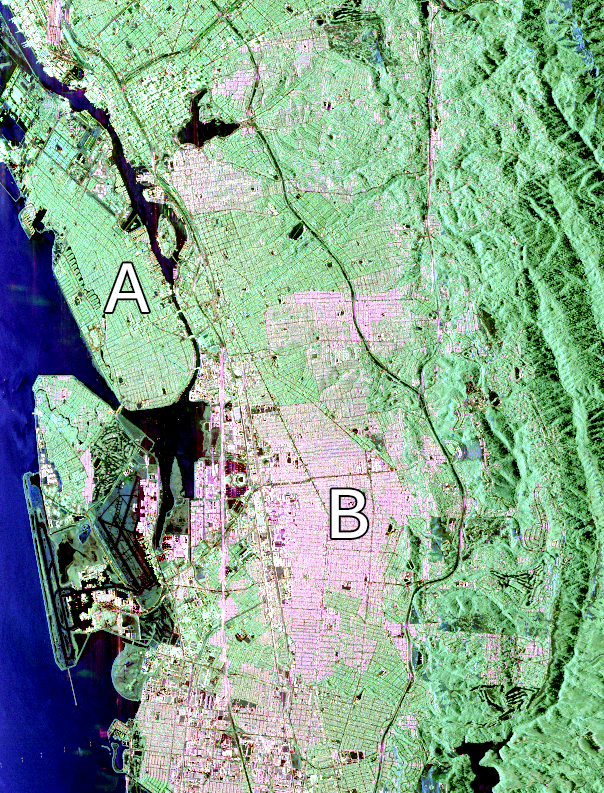
\includegraphics[width = 0.6\columnwidth]{Figures/Trento/ExampleOrientation}
%	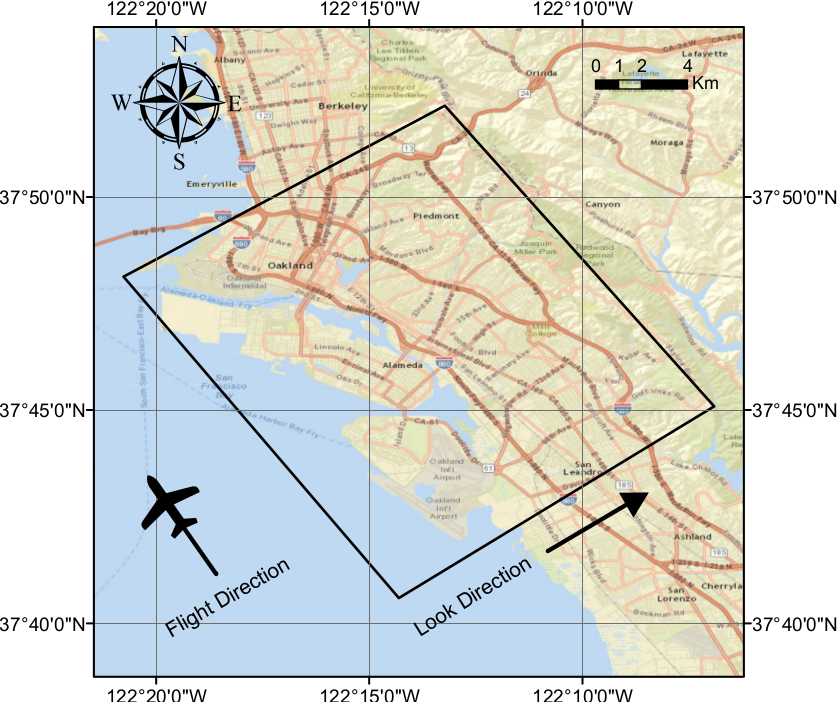
\includegraphics[width = 0.80\columnwidth]{Figures/Map} \quad
	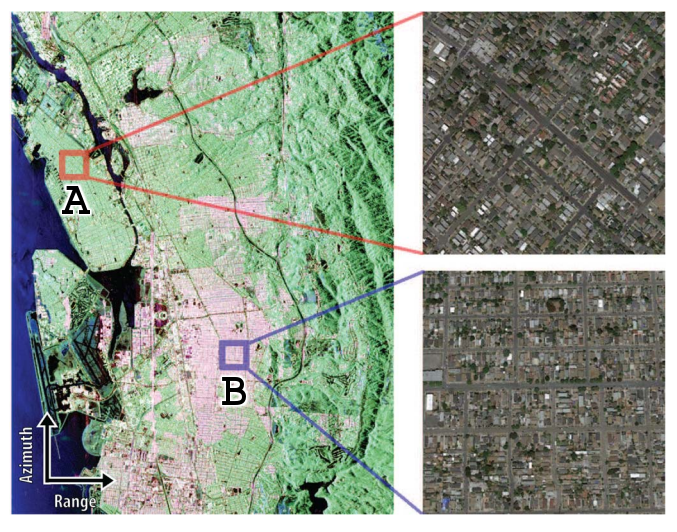
\includegraphics[width = 0.75\columnwidth]{Figures/Trento/UrbanProblem2}
	\caption[PolSAR orientation problem]{Pauli composite generated from UAVSAR polarimetric data-take acquired over Oakland, CA is show along with optical data from Google Earth. Area $A$ is oriented with the radar line of sight while area $B$ is not.}
	\label{fig:orientationExample}
\end{figure}


%DL algorithms
\begin{figure*}[!b]
\centering
		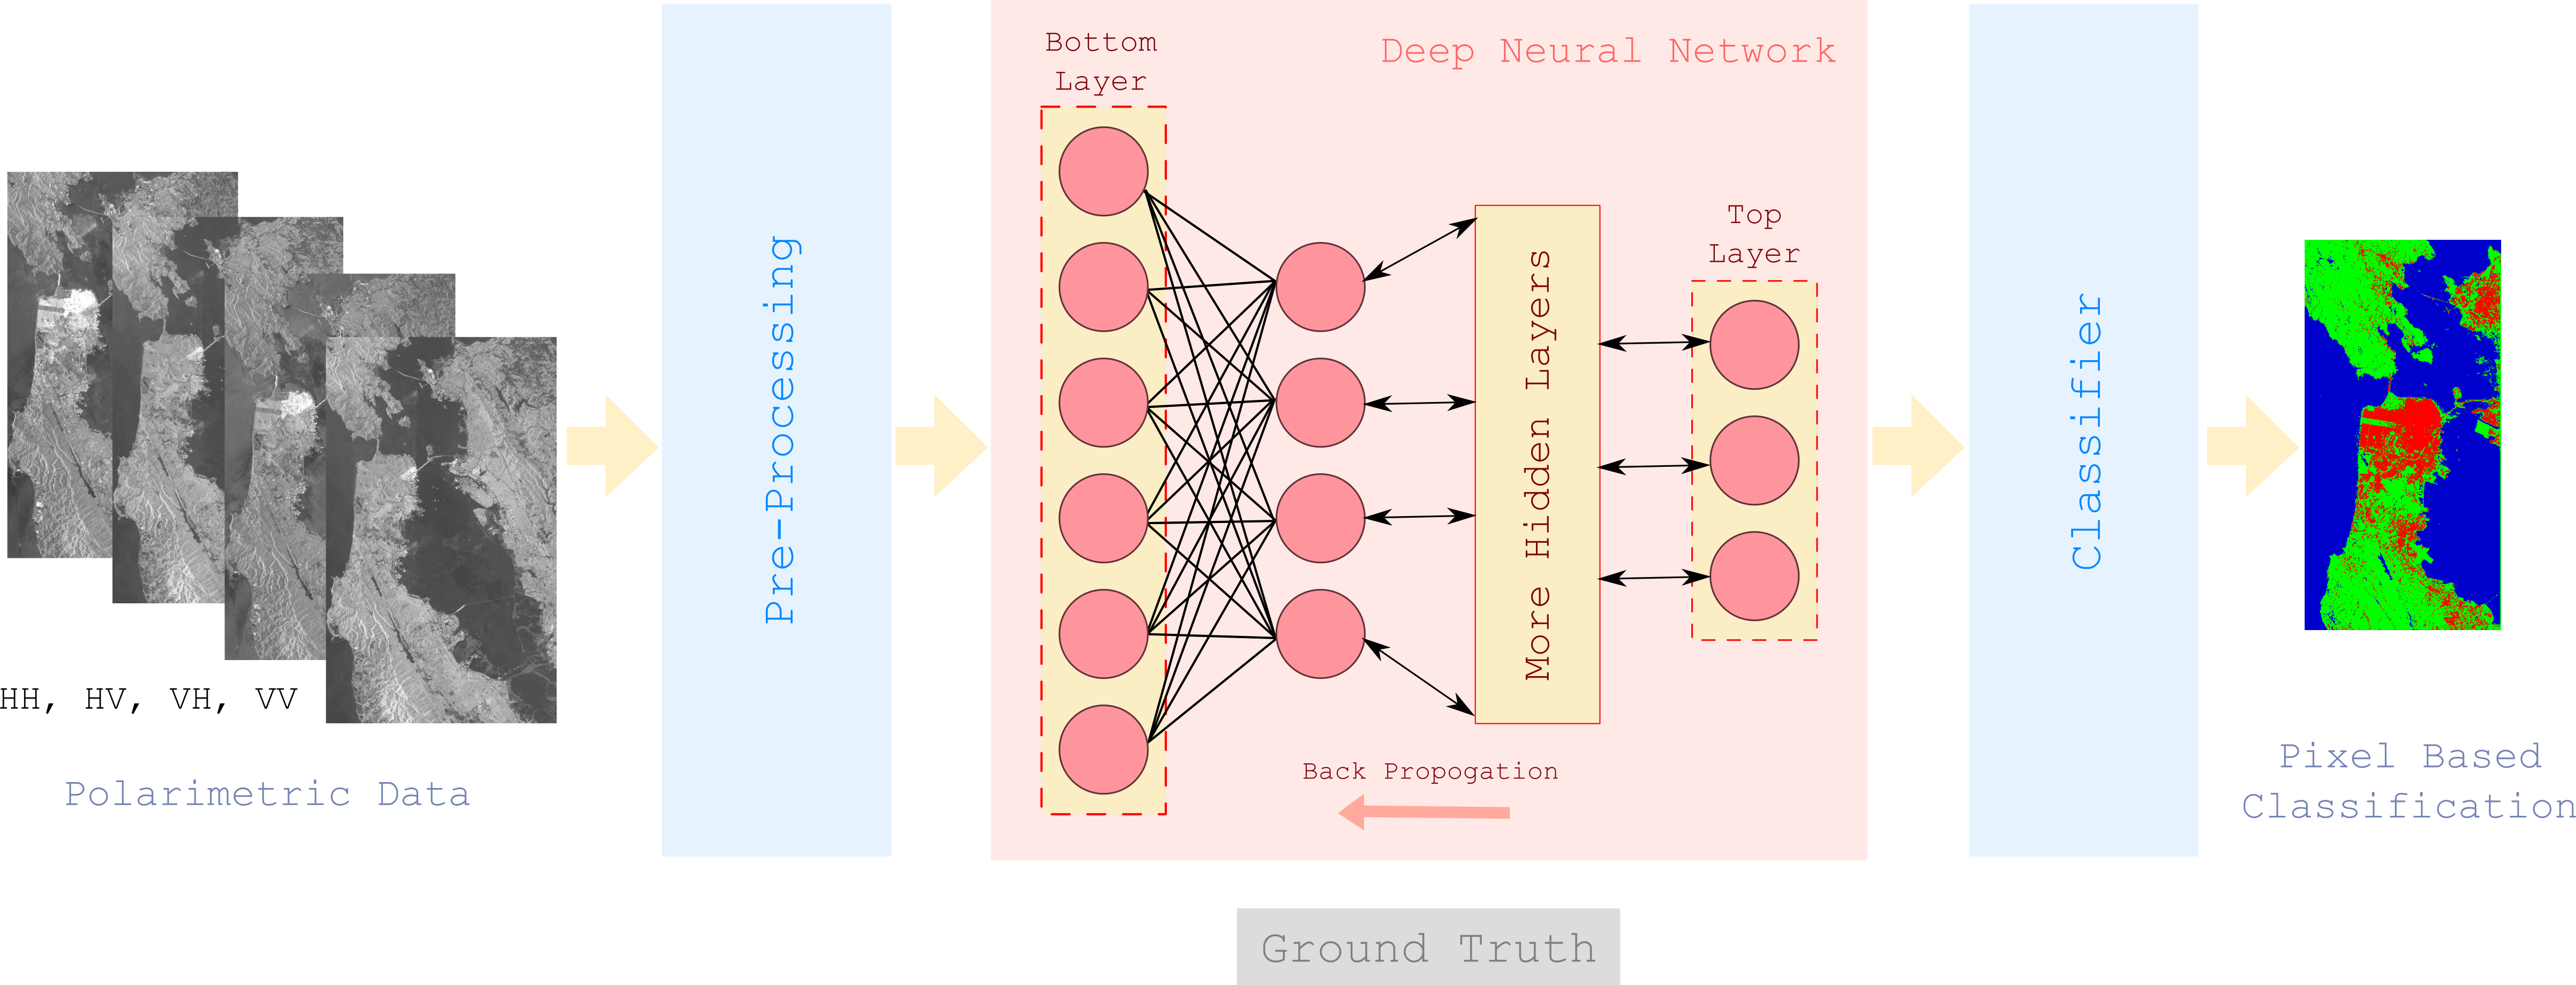
\includegraphics[width=0.75\columnwidth]{Figures/Trento/OverallDL}
		\caption{Framework for pixel classification of PolSAR images using a deep learning architecture.}
		\label{fig:GenDL}
\end{figure*}

%% Referenced in Methdology (introduction) to explain
%% the problem of rotation.
%% TO-DO: Add arrows in figure


%% Overall block diagram of the whole methodology
\begin{figure*}[!b]
	\centering
%	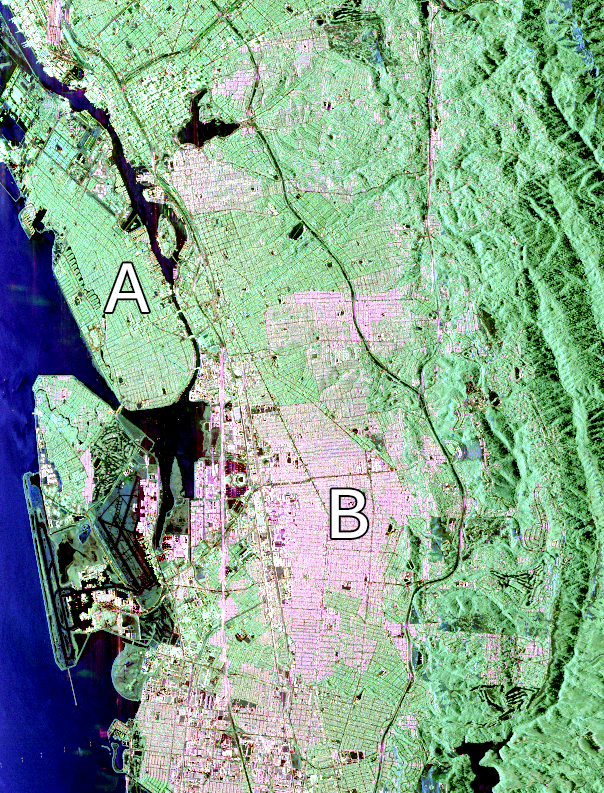
\includegraphics[width = 0.6\columnwidth]{Figures/Trento/ExampleOrientation}
	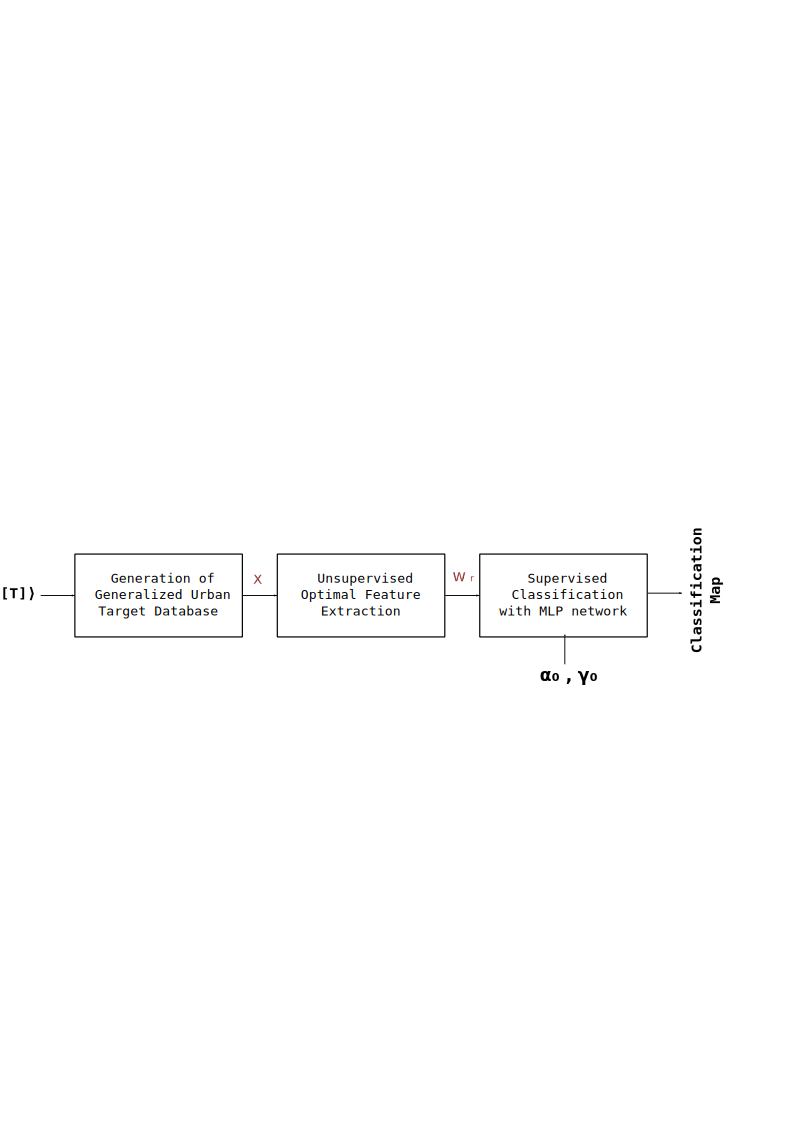
\includegraphics[width = 0.75 \columnwidth]{Figures/Trento/Method0}
	\caption[Overall Methodology]{ Block diagram of the proposed approach.}
	\label{fig:method0}
\end{figure*}

\begin{figure*}[t]
\centering
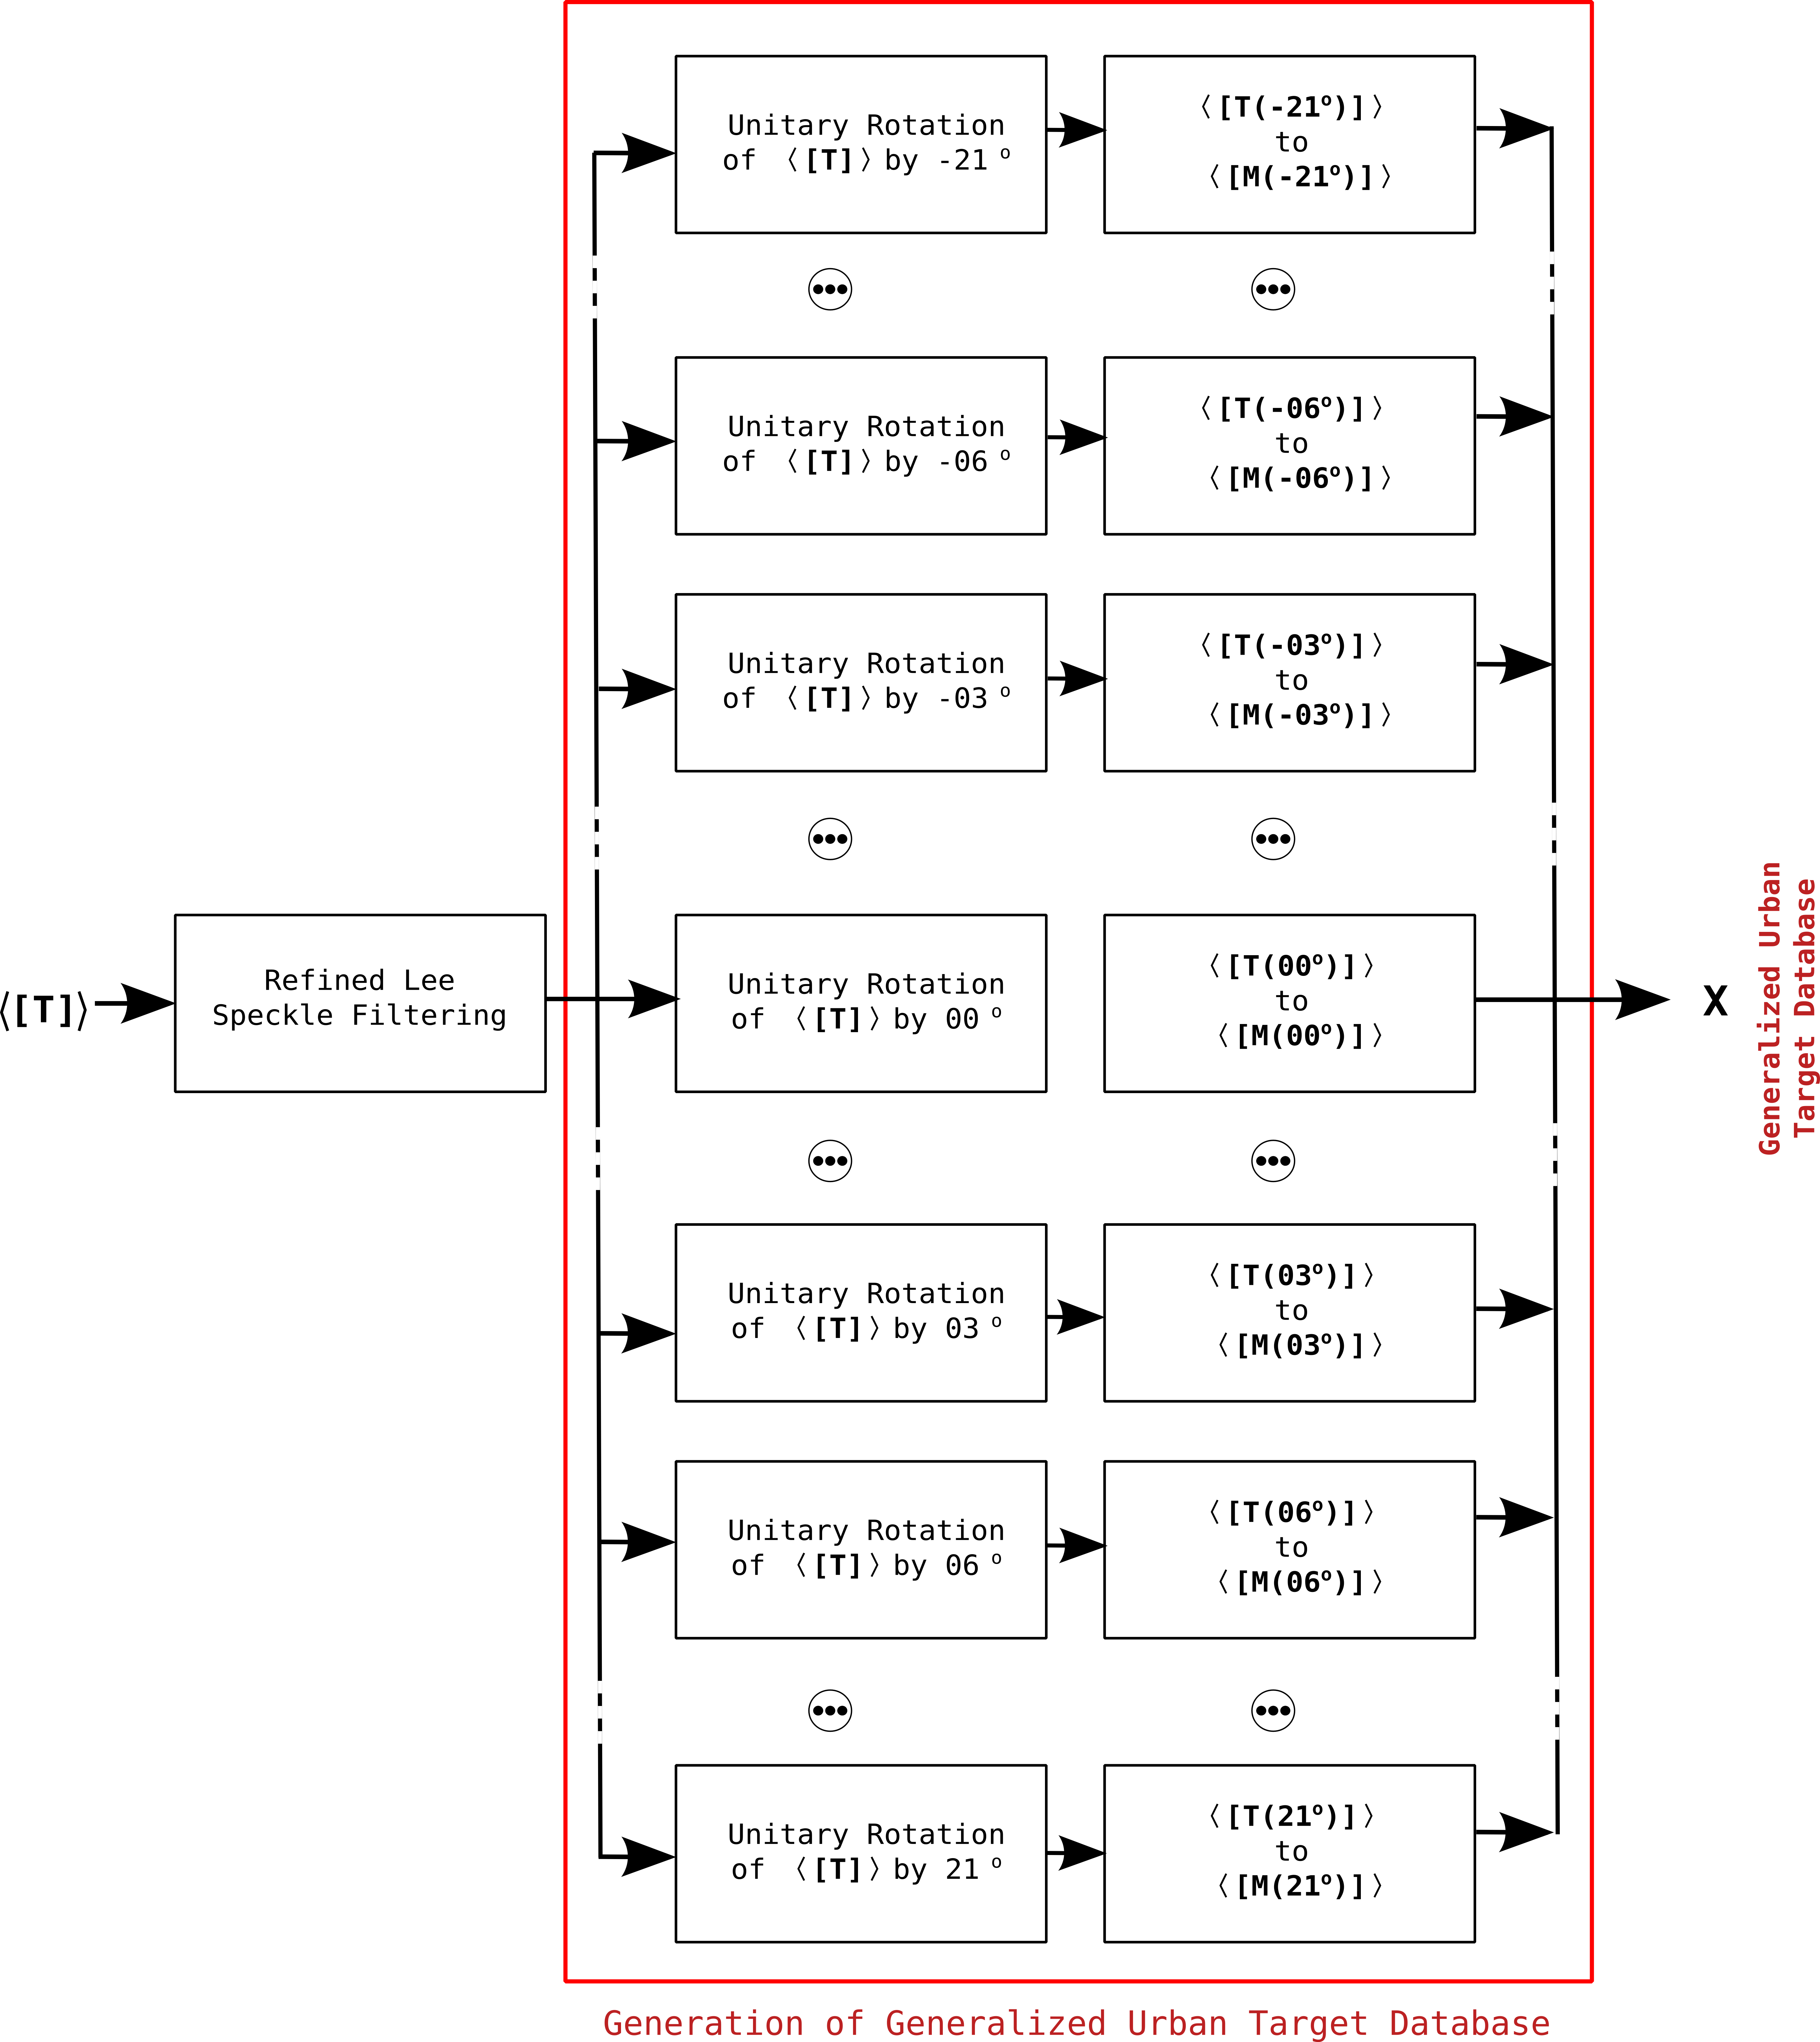
\includegraphics[width = 0.75\columnwidth]{Figures/Trento/Method1}
\caption[PolSAR data preprocessing]{Schematic diagram of the PolSAR data pre-processing and physics based generalized urban target database generation step.}
\label{fig:method1}
\end{figure*}

% % % % % % % % % % % % % % % % % % % % % % % % % %
%             End of Figures                      % 
% % % % % % % % % % % % % % % % % % % % % % % % % %

% % % taking out this header % % % %
%\section{Proposed Classification Approach}


The proposed approach for pixel classification of PolSAR data is shown in Figure~\ref{fig:GenDL}. The polarimetric channels can be considered as low-level input features that describe the geometry and dielectric properties of the target. However, these features are not robust enough to obtain accurate and stable classification performance. A pre-processing step is  applied to transform them  into more robust mid-level features, but this expands the data volume many-fold. A deep learning network is used to extract high-level features which are both efficient and robust with respect to the mid-level ones. In literature both supervised structures such as CNNs~\cite{hu2015deep} and unsupervised structures such as auto-encoders~\cite{chen2014deep}, DBNs~\cite{chen2015spectral} are used to this end. The mid- or low-level features are given as input to the network at the bottom layer and features are extracted from either the top or intermediate layers.  The  features are then classified using a suitable supervised classifier. In general, there are two kinds of classifiers. Hard classifiers such as SVMs which directly produce the classification label as output at every pixel, and soft classifiers such as logistic regression that can fine-tune the whole pre-trained network and predict the class labels as a probability.
The proposed method aims at classifying PolSAR images to identify urban areas and separate them from their surrounding land-cover classes, forest, bare-soil and water bodies. Segmented urban area maps can subsequently be used to characterize urban density, land-area usage, urban sprawl, and land cover change in temporal data amongst other applications. 

The difficulty in the classification of urban areas from PolSAR data arises because of the complex scattering of the polarized radar pulse from urban structures~\cite{kimura2008radar}. This is especially pronounced when they are oriented away from the radar line of sight. Range and azimuth slopes can cause the polarization to rotate about the radar line of sight, which causes the erroneous identification of the scattering mechanism. %~\cite{souissi2016analysis}. 
For instance, scattering observed from urban structures oriented away from the radar line of sight exhibit high cross-polarization as shown in Figure~\ref{fig:orientationExample}. This presents a confusion between urban areas and vegetation leading to incorrect classification. To overcome this challenge, a novel synthetic rotation based approach is proposed which simulates other rotated synthetic targets based on those present in the scene. This allows the machine learning algorithm to better generalize, be more robust and successful in discriminating oriented urban areas. 

The classification process consists of three stages as shown in Figure~\ref{fig:method0}. The first stage deals with the pre-processing of the PolSAR data and the generation of a generalized synthetic urban target database by transforming the input data to obtain a more general representation of the target (sub-section~\ref{sec:stage1}). The second stage is an unsupervised feature learning step, which automatically learns an optimal representation of the generalized database using a stacked auto-encoder network (sub-section~\ref{sec:stage2}). Finally, the third stage extracts optimal features from the previous stages, along with some statistical parameters and performs a supervised classification by using a multi-layer perceptron (MLP) network (sub-section~\ref{sec:stage3}). 



% \textcolor{red}{passive voice}we pre-process the PolSAR data. A refined Lee filter is applied for speckle suppression. To overcome the problem of targets oriented with respect to the radar line of sight, we synthetically rotate the input $\bm{T3}$ matrix to obtain a more general representation of the target, and store each of these rotated $\bm{T3}$ matrices. These are then converted to Mueller matrices and used in training the auto-encoder. As shown in subsequent sections, this helps the learning-machine identify urban targets of similar nature, but oriented with different angles, improving the accuracy of the final classification. In the first stage, the PolSAR data is pre-processed and synthetic rotations are applied. This step allows the simulation of targets rotated away from the radar line of sight, based on the targets that are present in the scene, allowing for increased generalization capability of the learning algorithm. The second stage consists of the auto-encoder which automatically learns an optimal feature representation from the input and synthetically generated data. Finally, in the third stage the features extracted from the preceding stage, along with some statistical parameters are classified in a supervised manner using a multi-layer perceptron (MLP) network. 



%----
\begin{figure*}[!htb]
\centering
	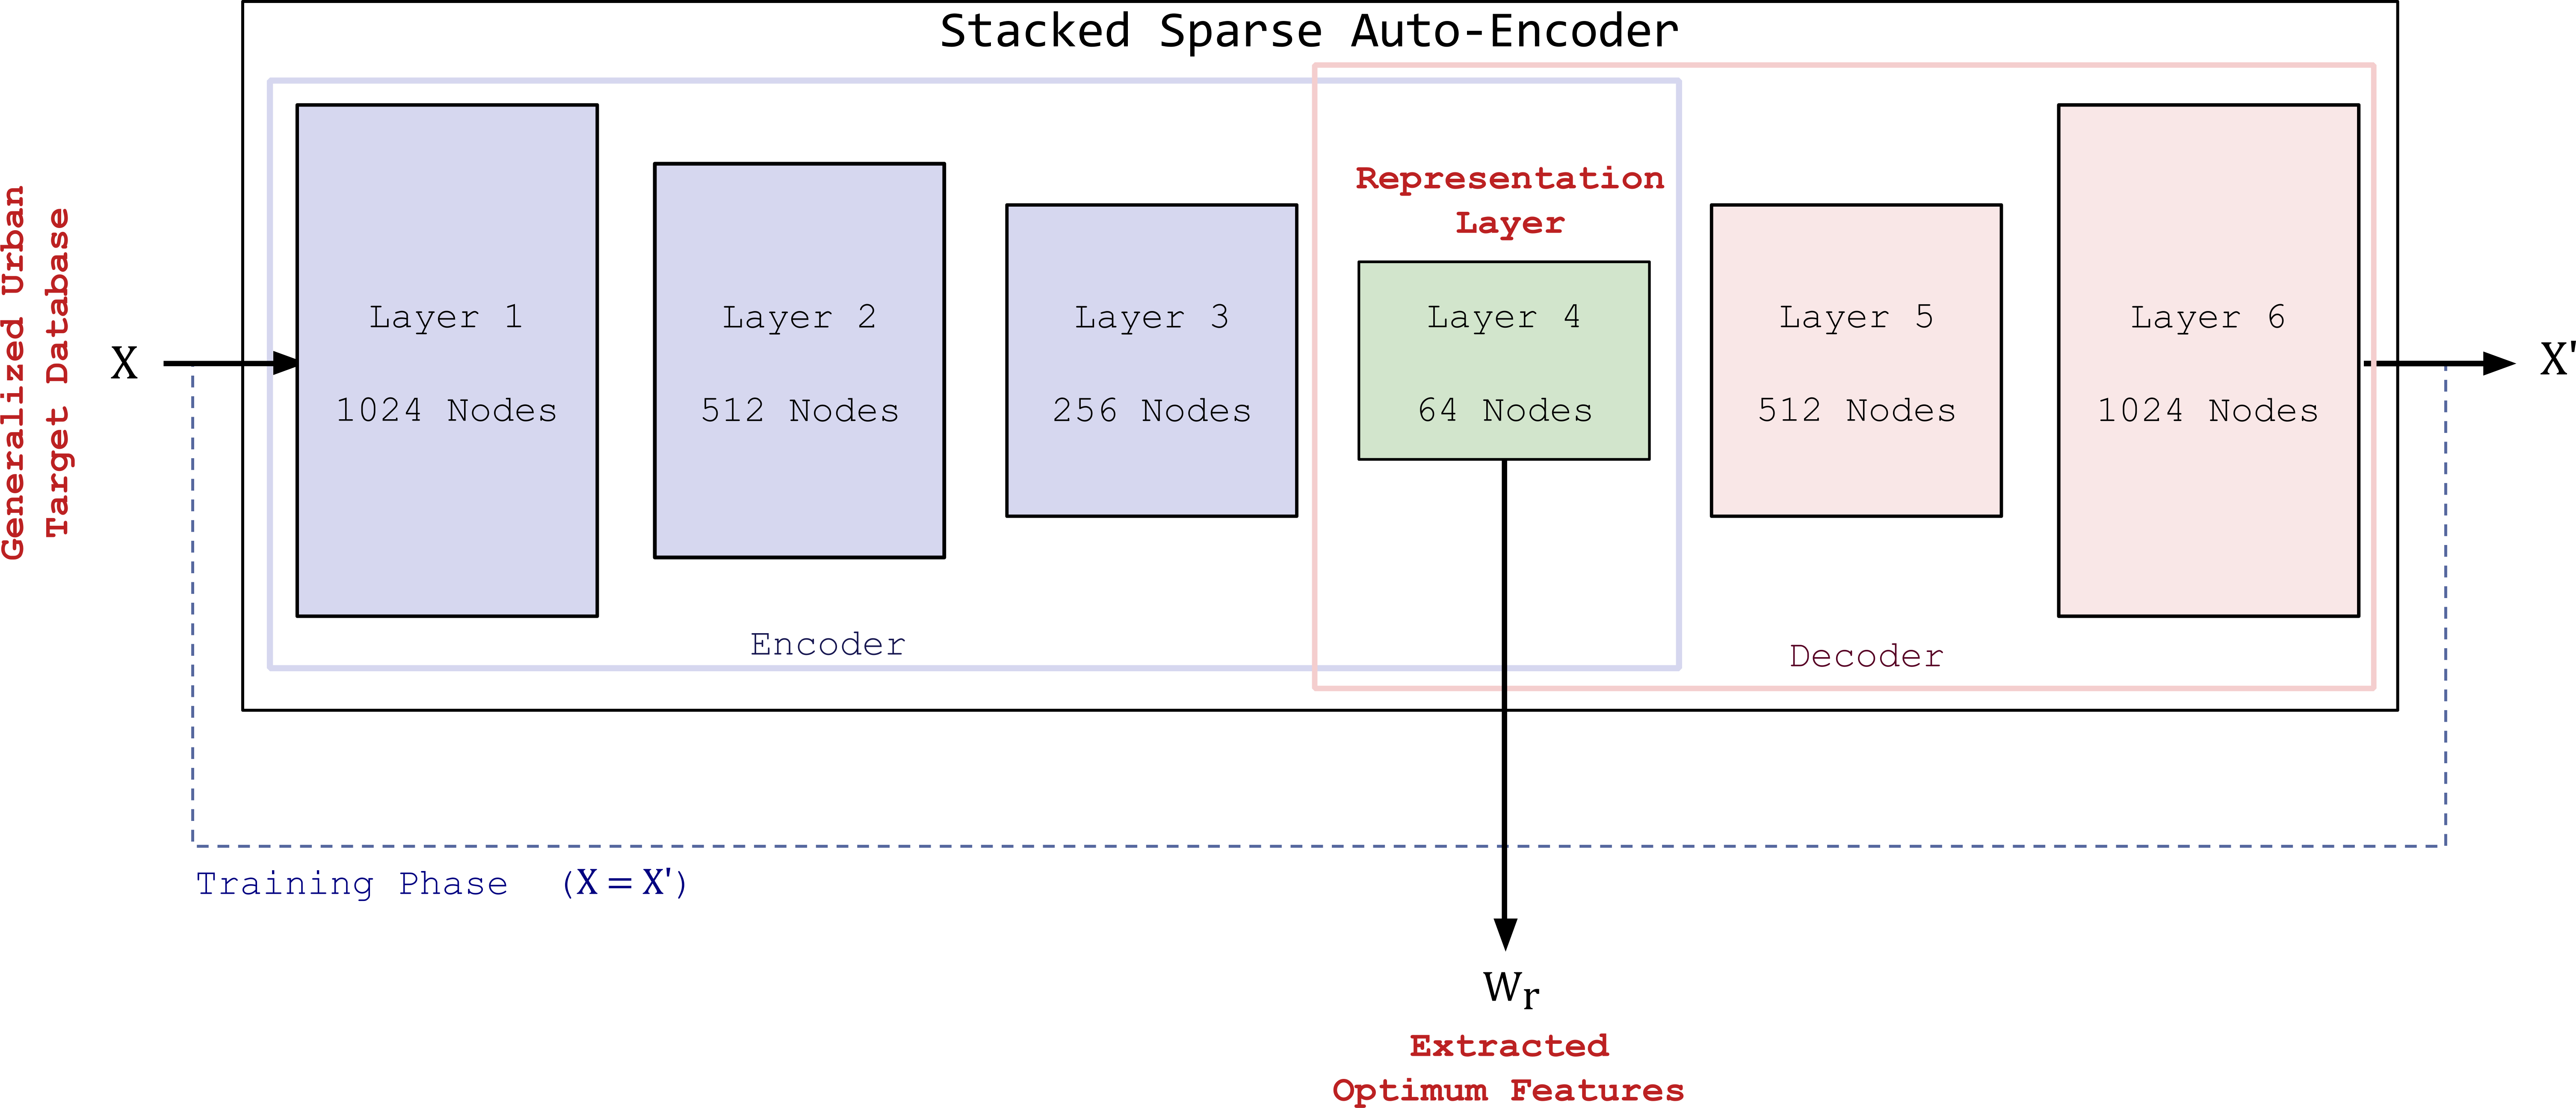
\includegraphics[width = 0.95\columnwidth]{Figures/Trento/Method2}
	\caption[PolSAR data preprocessing Stage 2]{ Auto-Encoder block scheme with Layer 4 extracted as the output feature-set. }
	\label{fig:method2}
\end{figure*}



	
%\subsection{Generation of Generalized Synthetic Urban Target Database}
\subsection{Data Preprocessing}
\label{sec:stage1}



%The first stage of the classifier is represented in Figure~\ref{fig:method1}. PolSAR data is made available from the sensor as a calibrated scattering matrix as described in Equation~\ref{eqn:scattring}. To utilize polarimetric information, we express the data as a spatially averaged coherency $\langle\bm{T3}\rangle$ matrix. Radar images, as a consequence of their coherent nature, are subject to a speckle pattern~\cite{lee1981speckle}. To suppress this, a Refined Lee speckle filter~\cite{lee1981refined} is applied to the dataset as a pre-processing step. This filter is based on the local statistics of the data, is effective, and has a good edge preservation ability allowing the retention of details~\cite{lee1994speckle}. The filtered $\bm{T3}$ matrix is then rotated by $\theta$ varying from $-22^\circ$ to $22^\circ$. Each rotated $\bm{T3}$ matrix is then converted to it's Mueller representation and the matrices are collated together for input to the next stage of the classifier. In this sub-section we describe the preprocessing applied to the polarimetric data, and the rotation based algorithm which is used to 


Measurement by a fully PolSAR system commonly involves the transmission of horizontally ($h$) and vertically ($v$) polarized radar pulses followed by their coherent reception. The polarization state of an incident electromagnetic wave is altered on scattering from a complex radar target. This alteration is a function of the physical and geometrical properties of the target itself, which in turn can serve to characterize it. This scattering  (or Sinclair) matrix is in the ($h,v$) polarization basis and has the form:


\begin{equation}
\mathbf{S} =
  \begin{bmatrix}
    S_{hh} & S_{hv}  \\
    S_{vh} & S_{vv}
  \end{bmatrix}
 \label{eqn:scattring}
\end{equation}


The full polarimetric scattering matrix is available for each imaged pixel and consists of four independent measurements ($hh$, $hv$, $vh$ and $vv$), with the phase relations between them recorded~\cite{tragl1990polarimetric}. Generally, in polarimetriy it is assumed that the targets are reciprocal. In the case of symmetric mono-static scattering, we can thus constrain the scattering matrix to be symmetric, \emph{i.e.} $S_{hv} = S_{vh}$. %The complex Pauli spin matrix basis set ${\{\Psi_P\}}$ can be written as,

%The three unique elements can be used to define a vector of the form: $
%\bm{u} ^\intercal = 
%\begin{bmatrix}
%S_{hh} & \sqrt{2}S_{hv} & S_{vv} \\
%\end{bmatrix}
%$. This vector, $\bm{u}$ has complex number elements. The term $S_{hv}$ is weighed by $\sqrt{2}$ to satisfy the condition that $|\bm{u}|^2$ = span(total power). 

 

%In most radar applications the target is susceptible to some temporal variation. If these variations occur over a time period larger then the illumination time of the radar, the target will appear to be relatively stable. Such targets are said to be deterministic or coherent. The scattering characteristics in this case can uniquely represented by the polarimetric scattering matrix ($\bm{S}$), which completely contains the information about the target at that radar frequency and scattering geometry. 

%However, if the period of the temporal variation is comparable to the observation time of the radar, the target is said to be incoherent or random. This is especially true of natural targets which can be thought of as a volume of a large number of particles moving in a random manner, and are therefore time dependent. Thus when illuminated by a monochromatic radar, the descriptors of the scattered wave, like the amplitudes $a_h(t)$, $a_v(t)$ and phases $\delta_h(t)$, $\delta_v(t)$ are also time dependent. The target thus can be considered to generate a quasi-monochromatic field variations of the scattered waves.  In this case, the target must be characterized by a time average of functions with integration time larger than typical periods of the target's fluctuations~\cite{cox1978ellipsometry}. 

%The Stokes vector representation or the covariance matrix~\cite{cox1978ellipsometry} can be used to describe the statistics of quasi-monochromatic waves. The Stokes formalism can be used to describe the target using the Mueller matrix, which can be related to the covariance matrix by linear transformations~\cite{cloude2009polarisation}.

% %

 
 
%\begin{equation}
%{\Psi_P = \left\{ \sqrt{2}   
% \begin{bmatrix}
%    1 & 0  \\
%    0 & 1
%  \end{bmatrix} 
%  \sqrt{2}   
%  \begin{bmatrix}
%      1 & 0  \\
%      0 & -1
%    \end{bmatrix} 
%    \sqrt{2}   
%    \begin{bmatrix}
%        0 & 1  \\
%        1 & 0
%      \end{bmatrix} 
%  \right\}}
%  \label{eqn:pauli}
%\end{equation}

%The factors $2$, $\sqrt{2}$ or $2\sqrt{2}$ are added in equation~\ref{eqn:pauli} to account for total power invariance with


%\begin{equation}
%Span(S) = |\bm{k}|^2 = |S_{hh}|^2 + 2|S_{hv}|^2 + |S_{vv}|^2
%\end{equation}


The corresponding $\bm{k_p}$-target vector is expressed as,

\begin{equation}
\bm{k_p} = \frac{1}{\sqrt{2}} \begin{bmatrix}  S_{hh}+S_{vv} && S_{hh}-S_{vv} && 2S_{hv} \end{bmatrix} ^T
\end{equation}
where the superscript $T$ denotes transpose. In the mono-static backscattering case, we can construct a $3\times3$ coherency matrix, $\mathbf{T}$, as

\begin{equation}
	\mathbf{T} =  \bm{k} . \bm{k}^{*T} 
\end{equation}


\begin{equation}
\mathbf{T} =  \begin{bmatrix}
t_1 & t_2 & t_3 \\
t_2^* & t_4 & t_5 \\
t_3^* & t_5^* & t_6 \\
\end{bmatrix} 
\end{equation}
where

\begin{align}
\begin{split}
\label{eqn:tmat}
t_1 &=  |k_1|^2   = \frac{1}{2} |S_{hh}+S_{vv}|^2 \\
t_2 &=  k_1k_2^*  = \frac{1}{2} |(S_{hh}+S_{vv})(S_{hh}-S_{vv})^*|^2 \\
t_3 &=  k_1k_3^*  =  (S_{hh}+S_{vv}) S_{hv}^*  \\
%t4 &= \langle k_2k_1^* \rangle = \frac{1}{2} \langle|(S_{hh}-S_{vv})(S_{hh}+S_{vv})^*|^2\rangle \\
t_4 &=  |k_2|^2   = \frac{1}{2} |S_{hh}-S_{vv}|^2 \\
t_5 &=  k_2k_3^*   =  (S_{hh}-S_{vv}) S_{hv}^*  \\
%t7 &= \langle k_3k_1^*  \rangle = \langle S_{hv}(S_{hh}+S_{vv})^* \rangle\\
%t8 &= \langle k_3k_2^*  \rangle = \langle S_{hv}(S_{hh}-S_{vv})^* \rangle\\
t_6 &=  |k_3|^2   = 2 |S_{hv}|^2  \\
\end{split}
\end{align}



$L$ independent and identically distributed samples are averaged to enhance the signal-to-noise ratio while forming the $3\times3$  $L$-looked $\mathbf{T}$ as,
\begin{equation}
\mathbf{T} =  \langle \mathbf{[T]} \rangle = \frac{1}{L} \sum_{i=1}^{L} \bm{k_{p_i}}.\bm{k_{p_i}}^{*\small T} 
\end{equation}
%The $3\times3$ polarimetric coherency $\mathbf{[T]}$ matrix is a Hermition positive semidefinite matrix. It can the transformed to the $3\times3$ polarietric covarience matrix $\bm{C_3}$ by linear unitary transformations~\cite{lee2009polarimetric}.
where $\langle ... \rangle$ denotes temporal or spatial ensemble averaging, under the assumption that the signal is ergodic. 
%and $N$ is the equivalent number of looks. 
Radar images, as a consequence of their coherent nature, are subject to a speckle pattern. Multilooking allows the exploitation of the second order statistical information while providing preliminary speckle suppression. A refined Lee filter~\cite{lee1994speckle} is applied to the dataset as a pre-processing step to further suppress speckle and improve classification performance. This filter is based on the local statistics of the data and has a good edge preservation ability allowing the retention of details.

%\subsubsection{Rotation of $\bm{T3}$} \label{sec:rotation}


The orientation of the target from the radar line of sight, or the presence of azimuth slopes can induce Polarization Orientation Angle (POA) shifts. These can lead to misinterpretation of the scattering characteristics of the target. This is especially common in urban areas oriented at an angle with respect to the radar line of sight and affects the classification performance. The rotation of the $\mathbf{T}$ can help to optimize and extract more polarimetric information which, in-turn helps to improve the characterization of the target scattering mechanism~\cite{bhattacharya2015adaptive}. 
If we consider a %diffused 
target which is symmetrical about the radar line of sight, the rotation of such a target about the radar line of sight can be represented by the unitary rotation of  $\mathbf{T}$ by a matrix rotation model expressed as
%. This can be expressed by transformation of the general averaged coherency $\mathbf{[T]}$ by a matrix rotation model as given by
%We can represent the effect of target rotation about the line of sight with the 
%Consider now a distributed target which has rotation symmetry around the line-
%of-sight as illustrated in Figure 3.10 [9].
%Consider initially a general form for the averaged coherency T 3 matrix and then
%consider transformation of this matrix to model rotations about the %line-of-sight. We
%then obtain the following expression for the averaged oriented coherency T 3 %(u) matrix:

\begin{equation}
\mathbf{T(\theta)} = \mathbf{R}(\theta) \mathbf{T} \mathbf{R}(\theta)^{-1}
\label{eqn:rotation}
\end{equation}

%\begin{equation}
%\mathbf{\langle[T(\theta)]\rangle} = %\mathbf{R}(\theta)\mathbf{\langle[T]\rangle}\mathbf{R}(\theta)^{-1}
%\label{eqn:rotation}
%\end{equation}
where the special unitary rotation matrix $\mathbf{R}(\theta)$ is given by

\begin{equation}
\mathbf{R}(\theta) = \begin{bmatrix}
1 & 0 & 0 \\
0 & \cos 2\theta & \sin 2\theta \\
0 & -\sin 2\theta & \cos 2\theta
\end{bmatrix}
\label{eqn:rotDeets}
\end{equation}
The orientation angle $\theta$ is estimated either by minimizing the $t_6$ element given in (\ref{eqn:tmat}) ~\cite{981347} or by  maximizing a  stochastic distance measure between the $t_6$ and the $t_4$~\cite{Bhattacharya2015}.  


Conversely, if the $\mathbf{T}$ matrix is rotated using unitary rotation as in~(\ref{eqn:rotation}), it would simulate the effect of physically rotating the target while measuring it with a polarimentric antenna. That is, the result of rotating the target $\mathbf{T}$ by $\mathbf{R}(\theta)$ is the $\mathbf{T}$ matrix that would be obtained with target having orientation $\theta$ from the radar line of sight during measurement. Thus, it is expected that by synthetically rotating and storing the rotated $\mathbf{T}$, we can generate a database of synthetic targets based on those detected in the scene.  The rotations are done in discrete steps as show in Figure~\ref{fig:method1} before being collated in a database. The granularity of the rotation steps is directly proportional to the size of training dataset and the capacity of generalization. If the rotations are closely spaced, the database will require more memory, but the generalization ability will be enhanced. However beyond a point, the gain in performance is not justifiable by the rise in computational cost. Therefore a step of $3^\circ$ is selected as a trade-off between performance gain and memory requirement, but other choices are possible. When these are used in the training of the learning algorithm, they improve the generalization capability of the network, allowing it to recognize targets with orientation not present in the original training data. Thus, the rotation based synthetic target database creation strategy in conjunction with a deep learning network architecture improves the classification accuracy of urban areas.

%\subsubsection{Mueller Matrix}
The $3\times3$ coherency matrix $\mathbf{T}$, which is hermitian by the nature of its construction, contains complex valued quantities in its off-diagonal elements. In the complex-number space the solution of differentiation is not guaranteed to be analytic. This poses a problem in the back-propagation step while using neural networks. An alternative approach would be to separate the real and imaginary parts of the elements of  $\mathbf{T}$ and use them as input for the network. However, splitting a complex number to process in real-valued neural networks leads to a sub-optimal representation of the domain of the problem~\cite{hirose2006complex}.
To get around it, we convert the complex valued $\mathbf{T}$ matrix to the real valued Mueller representation. 
%This prevents the direct use of back-propagation based machine learning algorithms like neural networks. 
The Mueller matrix $\mathbf{M}$ is a $4\times4$ real matrix, that can be obtained by a linear transformation of the $\mathbf{T}$ matrix as


% % TODO FOOTNOTE SOMEHOW
\begin{equation}
\mathbf{M} = 
\frac{1}{2} 
\begin{bmatrix}
t_1+t_4+t_6 & t_2+t_2^* & t_3+t_3^* & -i(t_5-t_5^*) \\
t_2 + t_2^* & t_1+t_4-t_6 & t_5+t_5^* & -i(t_3-t_3^*) \\
t_3 + t_3^* & t_5+t_5^* & t_1 - t_4 + t_6 & i(t_2 - t_2^*) \\
-i(t_5-t_5^*) & -i(t_3-t_3^*) & i(t_2 - t_2^*) & -t_1 + t_4 + t_6 \\
\end{bmatrix}
\end{equation}

$\mathbf{M}$ is a real valued matrix with $16$ elements, which reduces to $10$ unique real elements assuming reciprocity conditions.  
%The elements of the matrix can be wholly represented by real numbers, 
This property makes the representation suitable for the purpose of feature learning by neural network structures. Additionally the Mueller matrix is also closely related to the physical properties of a target~\cite{barakat1981bilinear}. This makes it a reasonable choice for identifying the scattering mechanism from targets. In this work, each rotated $\mathbf{T}$ matrix is thus converted to its $\mathbf{M}$ representation.  $\mathbf{M}$ matrices are then collated together as a database of synthetically generated generalized urban targets to serve as input to subsequent stages of the learning algorithm.



%Thus in this stage the input $\mathbf{[T_{3}]}$ matrix is synthetically rotated to simulate a variety of targets, then converted to its $\bm{M}$ representation. All generated $\bm{M}$ matrices are collated together to ease the process of input to subsequent stages of the learning algorithm.


%~\cite{SilvaWishart13}

%Jones to S
%Stokes to Jones
%Mueller and stokes

%Advantage of mueller / real numbers
%physical relation - scattering **




%Polarimetric syntheric Aparture Radar data is collected 
%Sar Data
%T3 or C3 matrix
%Rotation of T3 - multiple angles
%What do I mean by rotation

%Conversion to Mueller 
%Muller repn theory

%Training of Auto Encoder
%Network description
%Architecture

% % % % % % % % % % % % % % % % % % % % % % % % % % % % % % % % % % % % % % % % % % % % % % % % % % % % % % % % % % %



%\subsection{Unsupervised Feature Extraction with a Stacked Auto-Encoder Network}
\subsection{Unsupervised Representation Learning using Auto-Encoders} ~\label{sec:stage2}




%\subsection{Autoencoder} 

\begin{figure}[t]
\centering
	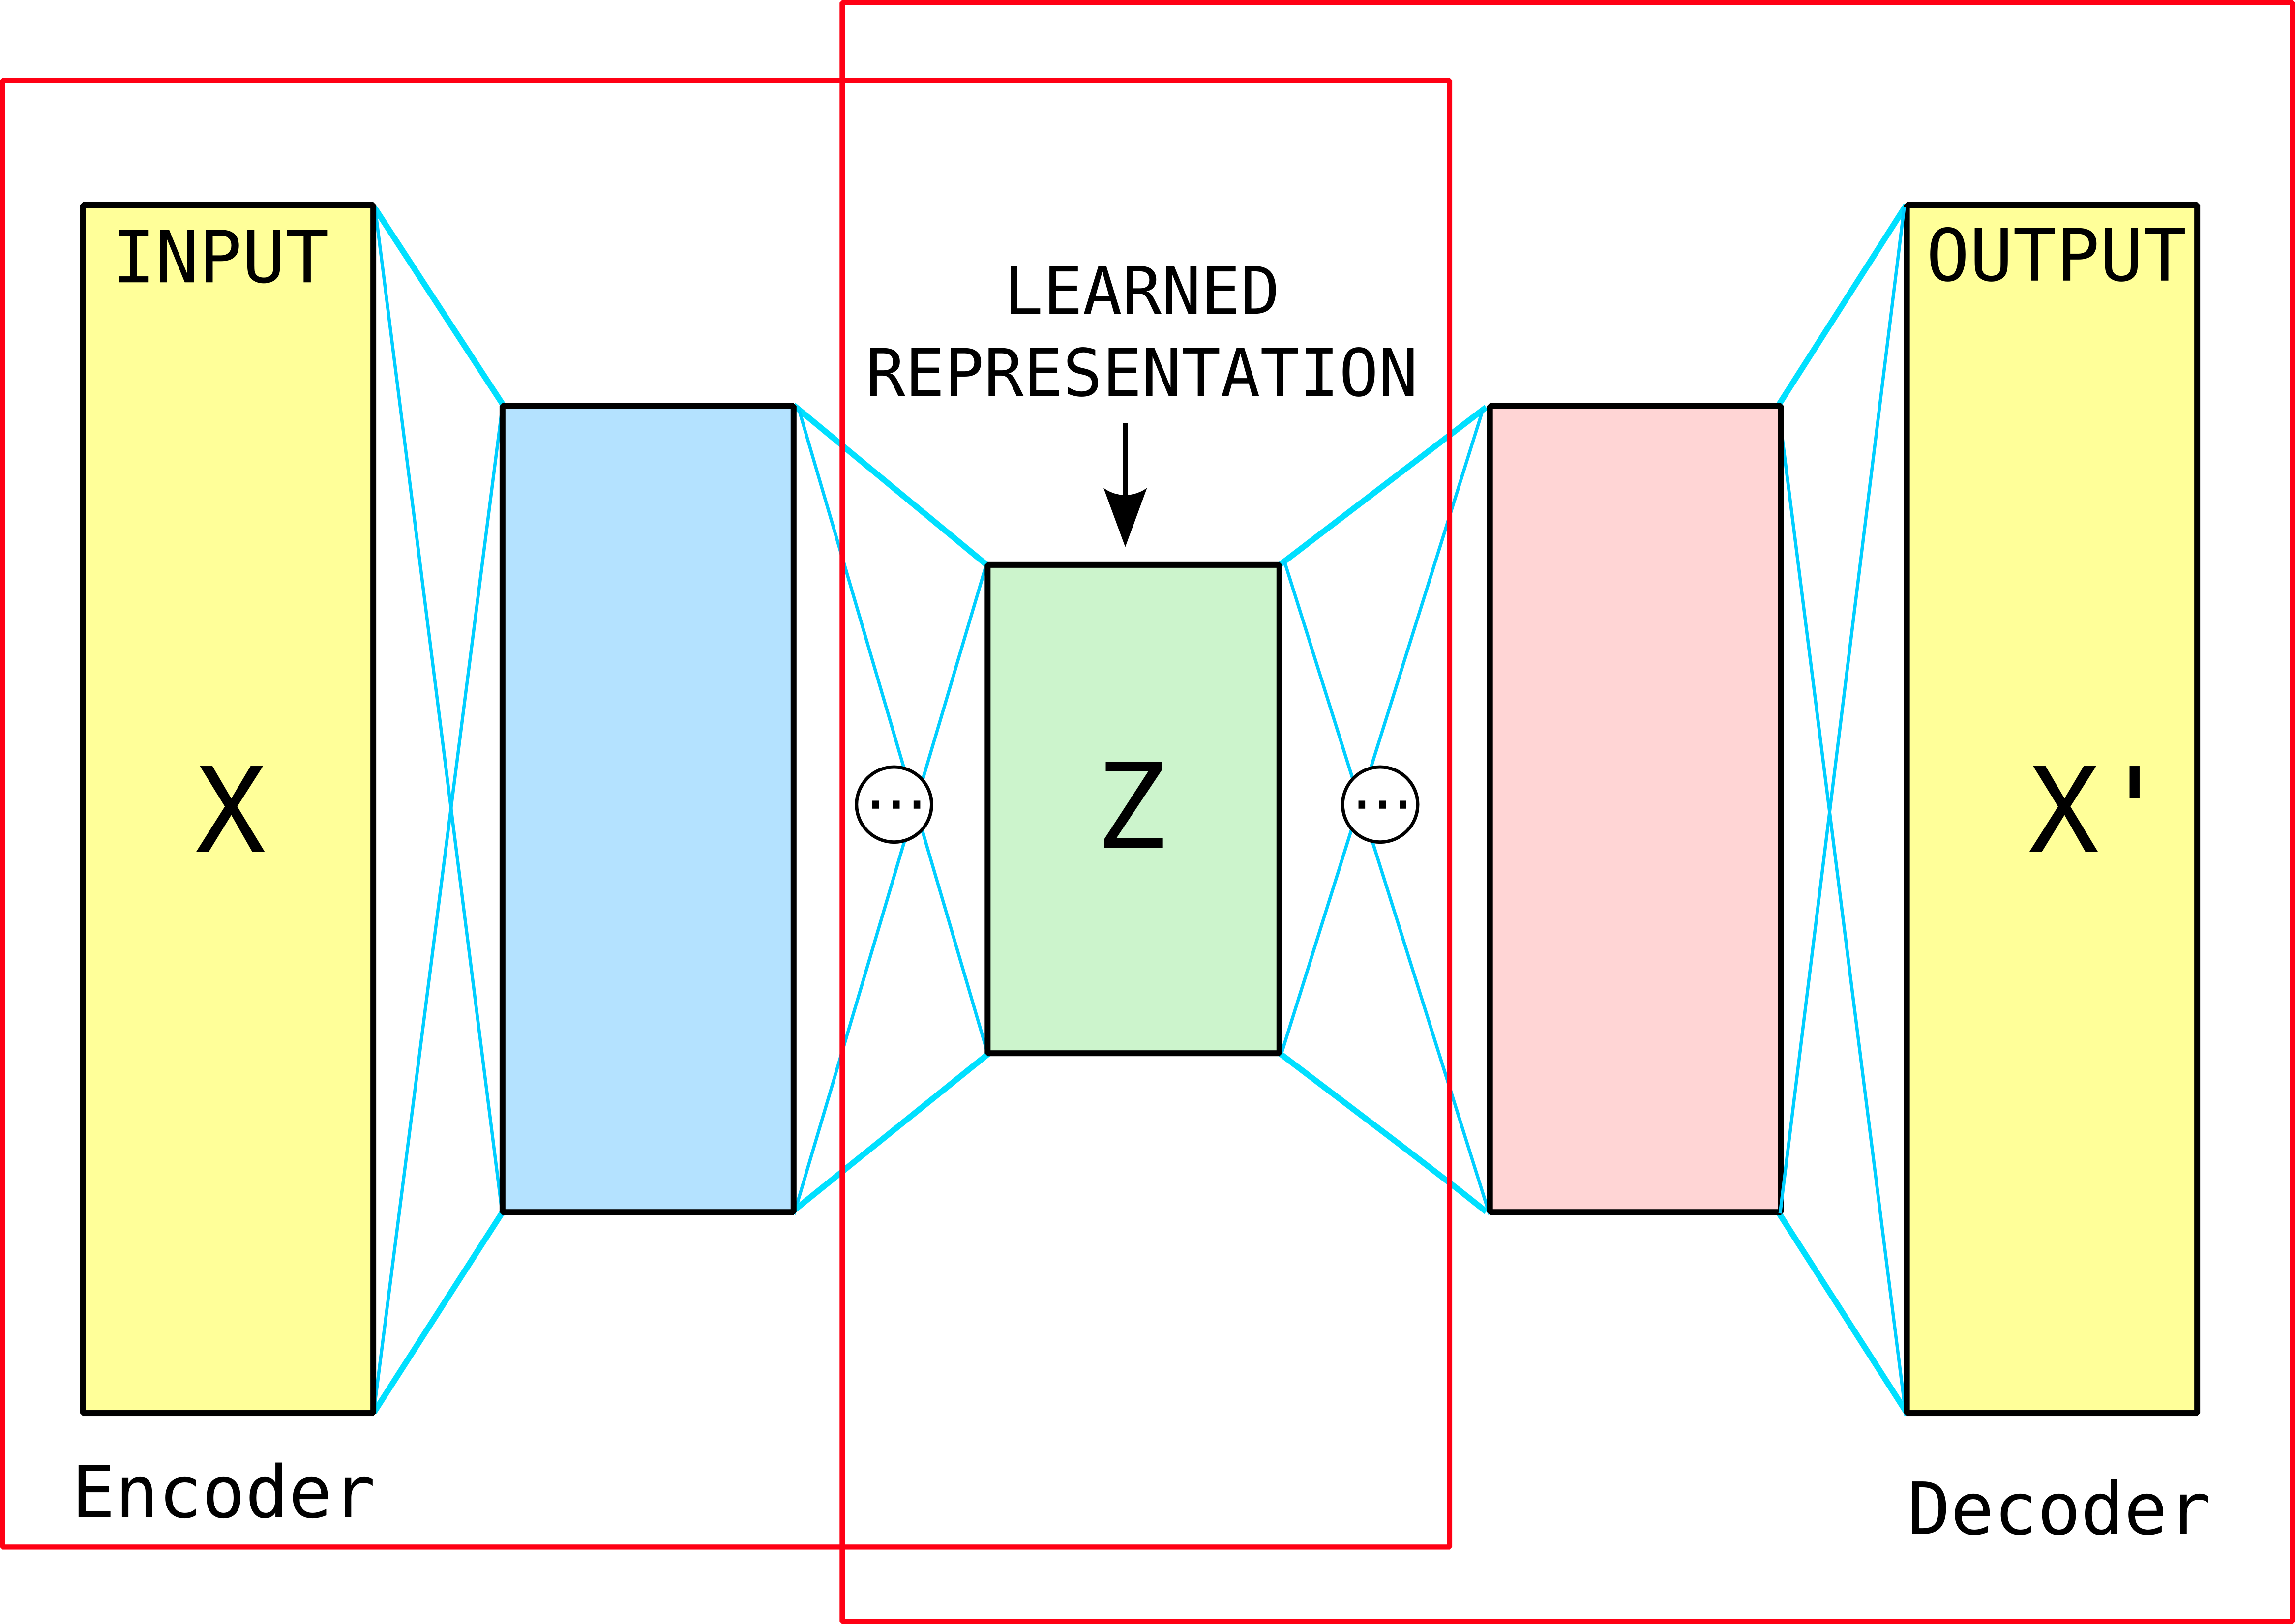
\includegraphics[width = 0.6\columnwidth]{Figures/Trento/AE}
	\caption[Schematic Diagram of an AE]{ Structure of a general auto-encoder with fully connected hidden layers. }
	\label{fig:AE}
\end{figure}

The second stage of the proposed classification method consists of an unsupervised sparse stacked auto-encoder (AE) which is represented in Figure~\ref{fig:method2}. An AE is a feed forward, fully connected, non-recurrent neural network with an input layer, an output layer and one or more hidden layers as shown in Figure~\ref{fig:AE}. 
The output layer has the same number of nodes as the input layer. During the learning phase the AE is trained to reconstruct for each pixel $i$ the input $X_i$ in the output $X'_i$
The error is back-propagated and minimized over multiple iterations. 

The collated synthetic urban target database from the previous stage is made available to the AE as input. The training is carried out  in an unsupervised manner. At the end of the training phase, the weights $W_r$ of the central hidden layer $Z$, are extracted to form an efficient feature representation of the dataset. This stage takes the $n\times10$ dimensional collated target dataset $X$, where $n$ is the number of synthetic rotations, and reduces it to an $m$ dimensional feature set $W_r$, where $m$ is the number of nodes in the representational layer $Z$ and $m < n\times10$. In practice the AE stage integrates information about the rotational response of the target and encodes it into a compact representation. Thus AE acts as an unsupervised feature learning stage and is able to automatically extract an optimized feature set from the input data. This self-learning of the features based on the training data is a hallmark of deep-learning based architectures. This step gives the network  greater generalization ability allowing it to respond to different orientation configurations of the targets. Thus once trained on a target that is  perpendicular to the radar line of sight, it can respond to the same target encountered at an orientation, even if such a configuration was not present in the training samples. %This ability is especially beneficial to classification performance in urban areas because targets, e.g. houses, are very similar in structure but differ in orientation to the radar line of sight. 
%The auto-encoder network used in this study is a 6 layer stacked sparse auto-encoder as shown in Figure~\ref{fig:method2}. The selection of the number of layers were done by training the UAVSAR data-set using the same hyper-parameters and number of nodes though different auto encoder topologies with increasing depth and measuring the lowest cross-entropy error achieved. This is plotted in figure~\ref{fig:layerplot}. We see that a 6-layer auto-encoder was found to be most optimal for this dataset. From input $x$ to output $y$, the network has $1024, 512, 256$ nodes in Layer 1, 2 and 3 respectively forming the encoder, and $128, 512, 1024$ nodes in Layer 4, 5 and 6 respectively forming the decoder. The non-linearity of each encoder is a Rectified Linear Unit (ReLU), allowing the handling of large dynamic range input without saturating.

To understand the action of the AE let us consider a learning problem where a labeled training set $(X_{i},l_{i})$ is available, where $X_i$ represents the input vector and $l_i$ is the corresponding label for the $i^{th}$ pixel. The label is not required for the unsupervised AE stage, but it is necessary for the subsequent classification. The  network consists of  individual neurons that are interconnected such that it is possible to define a complex, non-linear, non-parametric hypothesis $h_{W,b}(x)$.  $W$ is the weight matrix and $b$ is the vector of bias terms for the network. Both these parameters are fitted to the data over the training process. A neuron is a computational unit that takes as input $\bm{X}_i^{n} = X_1,X_2 ... X_n$ and an intercept term $b$, and produces the output, called hypothesis, $h_{W,b}(X) = f(\bm{W^{\intercal}x}) = f(\sum_{i=1}^{n}W_ix_i+b)$, where $f: \Re  \Rightarrow \Re $ is called the activation function or nonlinearity. 

Traditionally the sigmoid $\sigma(x) =  1 / (1+e^{-x})$  has been used as the activation function. It takes a real-valued number $x$ and returns a value within $[0,1]$, according to the magnitude of the input. In practice this has some drawbacks. The output of the sigmoid saturates at either tail of $0$ or $1$ and the gradient at these regions tends to zero, which causes a very small output to be back-propogated. Additionally, if the initial weights are large, the neuron can quickly become saturated during training. The sigmoid function also is not zero centered. During back-propogation if the input data to the neuron is always positive, i.e. $x>0$, then the gradient weights will either become all positive, or all negative. This could introduce undesirable oscillation dynamics in the gradient updates for the weights. To overcome the non-zero centering problem one may use the $\tanh$ activation function, $ f(x) = \tanh(x) = (e^x - e^{-x}) / (e^x + e^{-x})$ which has the limits $[-1,1]$. However this function is subject to saturation when the input has a large dynamic range as it is common in SAR data. 
A non-saturating nonlinearity like the Rectified Linear Unit (ReLU) activation function~\cite{glorot2011deep} can be used to overcome the saturation problem. The ReLU $f(x) = \max(\epsilon,x)$ simply thresholds the data at $\epsilon$, typically $\epsilon=0$. The differentiation of the function is defined as $ \frac{df}{dx} = \{1 : x > \epsilon, 0 : x < \epsilon\}$
%\[
%   \frac{df}{dx} = \left\{
%     \begin{array}{lr}
%       1 & : x > \epsilon\\
%       0 & : x \leq \epsilon
%     \end{array}
%   \right.
%\]  
Another advantage is that the training time for saturating activation functions is larger with the gradient descent algorithm than for its non-saturating counterparts~\cite{krizhevsky2012imagenet}. Since deep learning algorithms use several layers, faster training of ReLU units (as compared to sigmoid or $\tanh$) translates to multi-fold reduction in training times~\cite{nair2010rectified}. Also, the computation of the output of a ReLU is  simple as it does not involve evolution of exponentials like in the sigmoid and $\tanh$, allowing for in-place computation and requiring less computer memory. 
A disadvantage of ReLU units is that, when subjected to large gradients they can update their weights to such a state that they can not be activated by subsequent inputs. The neuron is said to 'die' in the training. To overcome this, the ReLU units can be modified to include a `leakage' term $\epsilon$, $f(x) = 1(x<\epsilon)(\alpha_r x) + 1(x \ge \epsilon)(x)$. This modification causes the units to have a small negative slope, $\alpha_r$ when the input is below the threshold, i.e. $x<\epsilon$. This allows the neuron to recover even if its weight has been updated to a high value by a particular input, over subsequent inputs. The differentiation can be defined as


\begin{displaymath}
   \frac{df}{dx} = \left\{
     \begin{array}{lr}
       1 & : x > \epsilon\\
       \alpha_r & : x \leq \epsilon
     \end{array}
   \right.
\end{displaymath}

The data must be given as input into the AE in random order to prevent it from memorizing the sequence in which the data are presented. The cross-entropy error in each iteration between the output of the AE and the input data is used to monitor the training. A progression towards zero indicates that the network is properly learning, while a stable value indicates that the learning stage is complete. The rate of adaptation of the network is determined by the set learning rate ($\alpha$). $\alpha$ is gradually reduced as the training progress. This is done by multiplying it by a set size multiplier ($\Gamma$). After a given number of iterations $\alpha$ is updated as $\alpha = \alpha \times \Gamma$.  The sparsity of the network is controlled by setting $\rho$, which is the expected activation of a hidden unit averaged across the training samples. As $\rho \rightarrow 0$ the representation becomes increasingly sparse, controlled by the adjustment of $b$. The performance of the stochastic gradient descent algorithm can be improved by introducing of a momentum term ($\mu$). Deep architectures tend to have steep slopes in the objective function near the local optima. This causes the gradient descent to oscillate and leads to a slow convergence. By introducing the $\mu$ term, these oscillations are dampened. 

The AE structure is now a close representation of the input data, and the internal nodes of the AE can be used as features in the classifier. The weights of the representation layer $\bm{W_r}$ of the AE are used as features after completion of the training phase. They are made available as input to the subsequent stage of the method. $\bm{W_r}$ is a sparse representation incorporating possible rotations of the targets present in the scene. This gives it a better generalization ability over the original data-space. A sparse representation also simplifies subsequent classifier design and improves accuracy due to improved inter-class separation~\cite{bengio2009learning}. 

\subsection{Supervised Classification} ~\label{sec:stage3}

\begin{figure}
\centering
	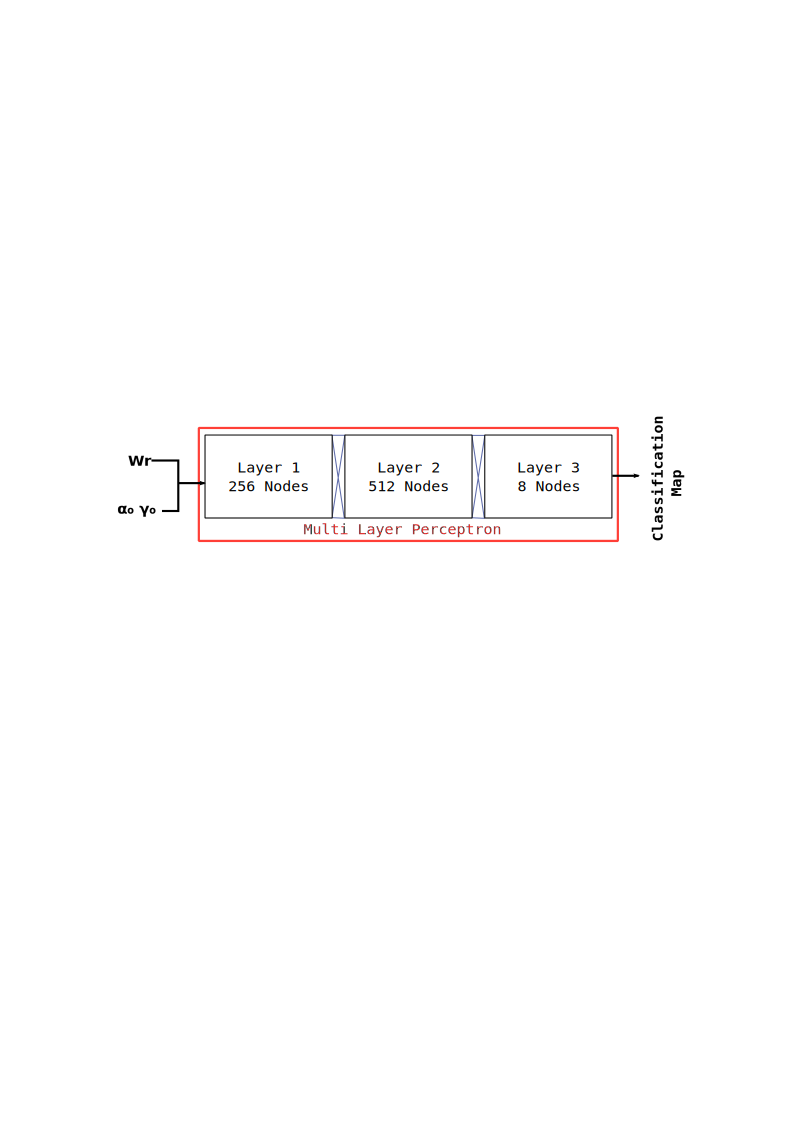
\includegraphics[width =  0.8 \columnwidth]{Figures/Trento/Method3}
	\caption[PolSAR data preprocessing Stage 3]{Stage 3: Final classification is done using a Multi-Layer Perceptron network with parameters extracted from the data.}
	\label{fig:method3}
\end{figure}
	

The third stage of the method consists of a multi-layer percepton (MLP) fully connected feed forward neural network (Figure~\ref{fig:method3}). The network is trained by a supervised learning algorithm that takes training data and labels as input and attempts to classify unlabeled additional unseen data-points. Here, the input to the MLP are the features $\bm{W_r}$ extracted from the previous stage and two statistical parameters $\alpha^0_{ij}$ and $\gamma^0_{ij}$ computed from the data. These parameters are generated by fitting the $\mathcal{G}^0_I$ distribution to the $hh$, $vv$ and $hv$ intensity bands~\cite{Frery97hetroclutter} over a moving window for each pixel ($i,j$) in the image. The three $\alpha^{pq}_{ij}$ and $\gamma^{pq}_{ij}$ parameters are averaged to compute the final values:
\begin{align}
\alpha^0 &= (\alpha^{hh}_{ij} + \alpha^{vv}_{ij} + \alpha^{hv}_{ij} )/3 \\ \label{eqn:stats}
\gamma^0 &= (\gamma^{hh}_{ij} + \gamma^{vv}_{ij} + \gamma^{hv}_{ij} )/3  \notag 
\end{align}
Here $pq$ represents the individual polarization bands ${hh,hv,vv}$ and parameters $\alpha^{pq}_{ij}$ and $\gamma^{pq}_{ij} \in \mathbb{R}$. These statistical parameters add textural context to the classification step improving the accuracy. The $\alpha^0_{ij} < 0$ serves as a measure of the homogeneity (smoothness) of the area while the  $\gamma^0_{ij}$ is the scale parameter of the distribution and thus is related to the brightness of the area~\cite{frery1999models}. For values of $\alpha^0_{ij}$ near zero, the imaged area is very heterogeneous, as in the case of urban areas. The value of $\alpha^0_{ij}$ diminishes to its lowest value for homogeneous areas. The parameter $\gamma^0_{ij}$ can help further discriminate between various type of targets.



The training labels are derived from ground truth information about the area. 
%A small fraction of the total pixels in the scene are used for training to prevent over-training of the neural network. 
%Care is taken to ensure that the training set is representative of the proportions of the land-cover in the scene. 
A three layer network is used to generate the final classification. The network weights and biases are randomly initialized at each iteration using the `Xavier' strategy~\cite{glorot2010understanding}. Since the inputs to this stage have smaller dynamic range, and because the goal is to classify the data into labels, we use sigmoid saturating nonlinearities.   
The network undergoes a training phase using the  labeled samples, extracted features and the statistical parameters. It is iterated to maximize the training accuracy on the test samples. Once the network weights are finalized, the unlabeled pixels in the dataset are classified to generate the  thematic map. 
%In the subsequent section, experimental setup of the methodology, justification for the choice of hyper-parameters and examination of the action of the encoder on the synthetic target database is presented. 
%A three layer network with $256$ hidden nodes in the first layer, $512$ in the second and $8$ in the final layer is used for the final classification. 
